\chapter{Limitations of existing protection Philosophies}



In a power system, a fault is an abnormal condition in which current flows outside its intended path, typically due to insulation failure or conductor issues. Faults may involve short circuits, causing high currents, or open circuits, which interrupt the flow. They often result from equipment malfunctions, human errors, or external factors and can cause outages, equipment damage, or safety risks. They result in outages of a specific asset or the entire network (e.g., a line, transformer, reactor, bus, generator, or load).

% \begin{figure}[!ht]
% \centering
% 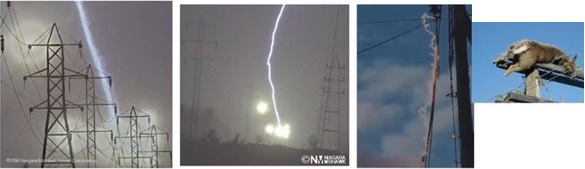
\includegraphics[scale=0.9]{images/chapter_1/Ch1F8.jpg}
% \caption{Faults in power system.}
% \label{Fig:ch_1_vieu}
% \end{figure}


\subsection{Classification of Faults}

Power system faults are broadly classified into \textbf{series (open conductor)} and \textbf{shunt faults}, based on the nature of the circuit abnormality.
Series or \textbf{open conductor faults} occur when one or more phase conductors break or disconnect, resulting in current interruption, voltage rise, and phase unbalance.
Shunt faults involve unintended connections between conductors or between conductors and ground, and are further categorized as \textbf{symmetrical} or \textbf{unsymmetrical}.

\begin{itemize}
\item \textbf{Symmetrical Faults:} All three phases are short-circuited, either with or without ground involvement (three-phase or three-phase-to-ground faults).
They are balanced in nature and, although rare (approximately $2$--$5$\% of all faults), produce the most severe fault currents.

\item \textbf{Unsymmetrical Faults:} These faults cause unequal currents in different phases and include the following types:
\begin{itemize}
\item \textbf{Single Line-to-Ground (L--G) Faults:} One phase shorted to ground, resulting in high zero-sequence current.
They represent nearly $70$\% of all faults, making them the most common.
\item \textbf{Line-to-Line (L--L) Faults:} Two phases shorted together without ground involvement, producing significant negative-sequence currents.
Occur in approximately $10$\% of cases.
\item \textbf{Double Line-to-Ground (L--L--G) Faults:} Two phases shorted together and to ground, exhibiting both L--L and L--G characteristics.
Their frequency of occurrence is around $10$--$15$\%.
\end{itemize}
\end{itemize}

In addition to the conventional classification of faults as \textbf{series (open conductor)} or \textbf{shunt faults}, and as \textbf{symmetrical} or \textbf{unsymmetrical}, faults can also be categorized according to several other engineering aspects.
These additional classifications help in understanding the nature of the fault, its impact on the network, and the type of protection required for reliable system operation.

\begin{itemize}
%---------------------------------------------------------
\item \textbf{Based on Duration:}
\begin{itemize}
\item \textbf{Transient Faults:} Temporary in nature and clear automatically once the cause (such as lightning or flashover) is removed.
Protection schemes may trip and reclose after a short interval to restore service.
\item \textbf{Permanent Faults:} Persist until the faulty section is isolated or repaired.
Caused by equipment failure, broken conductors, or persistent insulation breakdown.
\end{itemize}

%---------------------------------------------------------
\item \textbf{Based on Nature of Connection:}
\begin{itemize}
\item \textbf{Grounded Faults:} Involve one or more phases making contact with the ground.
Examples include L--G or L--L--G faults.
\item \textbf{Ungrounded Faults:} Occur between conductors without any ground connection, such as L--L faults.
\end{itemize}

%---------------------------------------------------------
\item \textbf{Based on the Equipment or Location Involved:}
\begin{itemize}
\item \textbf{Generator Faults:} Internal short circuits or stator winding faults leading to unbalanced operation or damage.
\item \textbf{Transformer Faults:} Winding-to-winding or winding-to-ground faults, core insulation failures, or bushing breakdown.
\item \textbf{Transmission Line Faults:} Commonly caused by lightning, pollution, or external contact with conductors.
\item \textbf{Busbar Faults:} Result from insulation failure or metallic flashover at switchyards and substations.
\end{itemize}

%---------------------------------------------------------
\item \textbf{Based on System Response:}
\begin{itemize}
\item \textbf{Active Faults:} Associated with a conducting path and flow of fault current (e.g., short circuits, ground faults).
\item \textbf{Passive Faults:} Do not involve current flow directly but alter system parameters, such as open circuits or overheating conditions.
\end{itemize}

%---------------------------------------------------------
\item \textbf{Based on the Cause of Initiation:}
\begin{itemize}
\item \textbf{Natural Faults:} Arise due to lightning strikes, wind, storms, or environmental effects.
\item \textbf{Human-Induced Faults:} Caused by operational errors, accidental contact, or maintenance oversights.
\item \textbf{Equipment Faults:} Originating from aging, insulation deterioration, or manufacturing defects.
\end{itemize}
\end{itemize}



The severity and type of fault determine the fault current magnitude, voltage unbalance, and system transients, all of which guide the protection design.





% \begin{figure}[!ht]
% \centering
% \includegraphics[scale=0.1]{images/chapter_1/faultclassification.pdf}
% \caption{Classification of Faults}
% \label{Fig:ch_1_vieu}
% \end{figure}


 
 
 \section{Power System Protection}

The primary philosophy of power system protection is to isolate faulty sections quickly and selectively while maintaining system stability and continuity of supply. A protection system detects this event using measured current and voltage waveforms. Protection aims to ensure:

\begin{itemize}
\item \textbf{Safety of personnel and equipment}
\item \textbf{Reliability, ensuring correct operation under all expected fault conditions}
\item \textbf{Selectivity, operating only for faults within its zone}
\item \textbf{Speed, minimizing fault duration and system damages}
\item \textbf{Sensitivity, detecting low-magnitude faults effectively}
\end{itemize}

% \begin{figure}[!ht]
% \centering
% 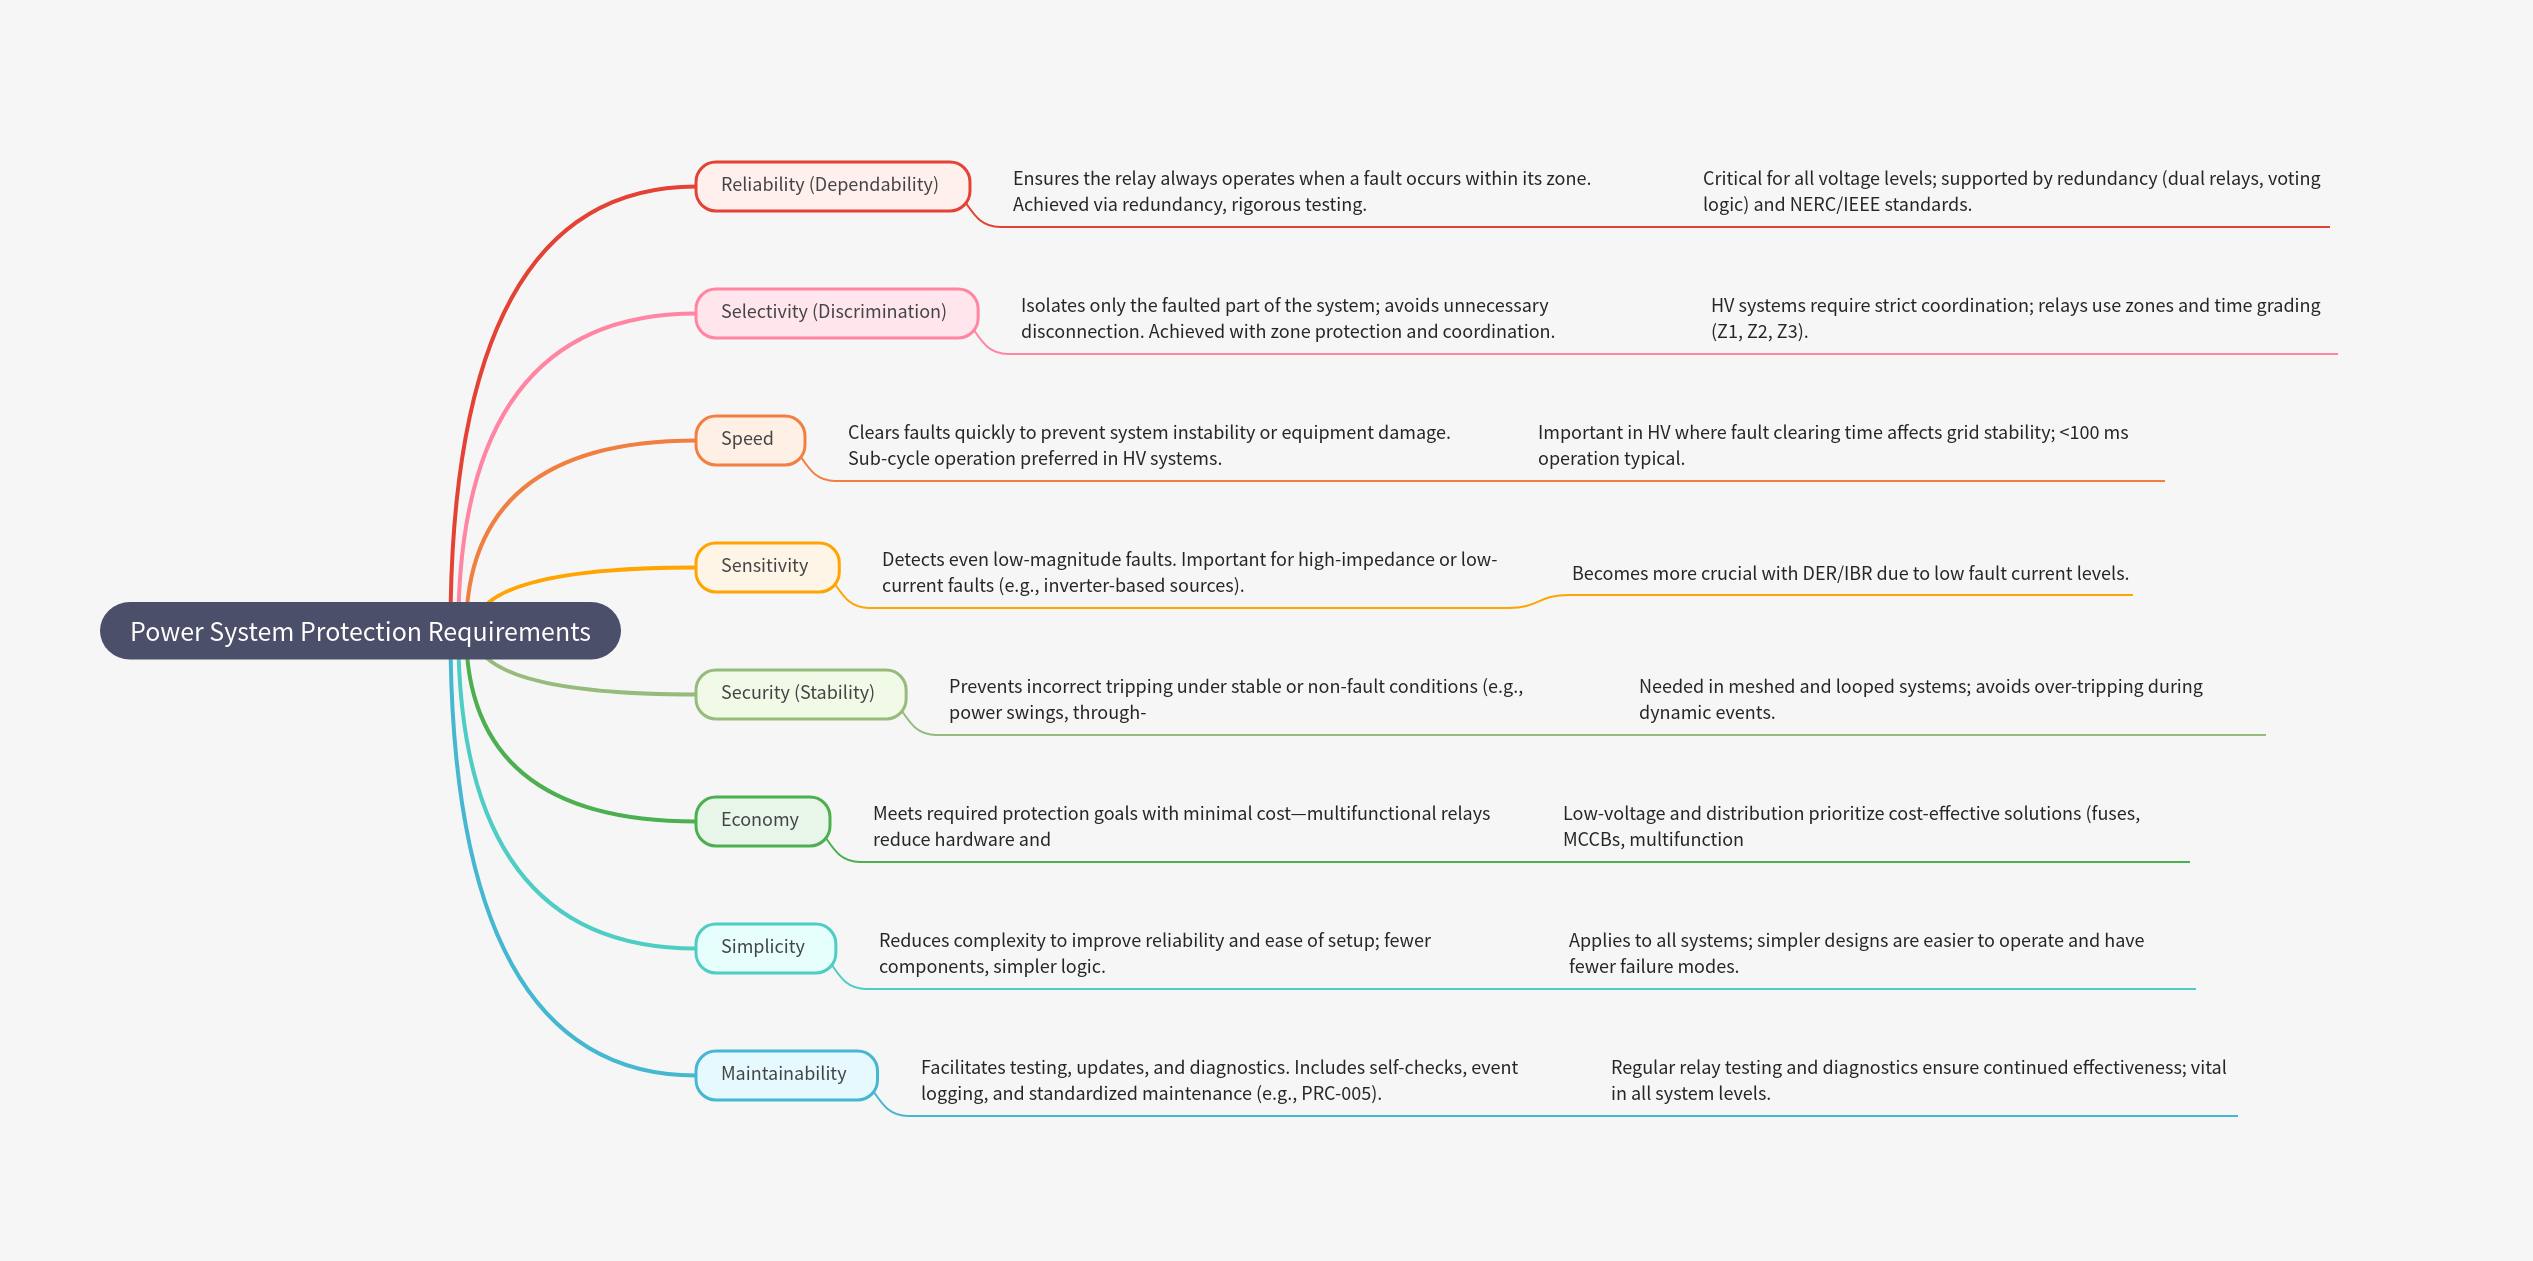
\includegraphics[scale=0.15]{images/chapter_1/PowerSystemProtectionRequirements.png}
% \caption{Power System Protection Features.}
% \label{Fig:ch_1_vieu}
% \end{figure}


In modern grids, this philosophy has evolved from radial logic to adaptive, communication-assisted frameworks capable of handling bidirectional power flows and inverter-dominated sources.
\section{Conventional relaying principles}

 \subsection{Relay Architecture}
A protective relay is an intelligent device designed to sense abnormal conditions and initiate tripping commands. A modern relay architecture typically comprises:

\begin{itemize}
\item \textbf{Measurement Unit}: processes input currents and voltages through CTs and VTs.
\item \textbf{Decision Logic}: compares the measured quantities against set thresholds using phasor or time-domain algorithms.
\item \textbf{Output Interface}: sends trip signals to circuit breakers.
\item \textbf{Communication and SCADA Interface}: enables coordination via IEC 61850, GOOSE messaging, and wide-area control.
\end{itemize}

The evolution from electromechanical relays to numerical and digital relays has enabled multi-functionality, event recording, self-diagnosis, and adaptive protection logic.

\begin{figure}[!ht]
\centering
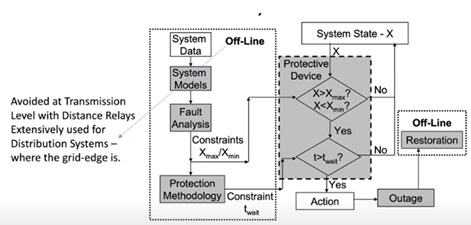
\includegraphics[scale=1.2]{images/chapter_1/Ch1F7.jpg}
\caption{Protection relay- as a function.}
\label{Fig:ch_1_vieu}
\end{figure}


\begin{itemize}
\item \textbf{Inputs}: Analog CT/VT signals; digitized using ADCs.
\item \textbf{Processing Unit}: Microprocessor/DSP runs protection logic and self-monitoring.
\item \textbf{Outputs}: Relay contacts trip breakers or signal alarms.
\item \textbf{Communication}: Supports IEC 61850, GOOSE,
SCADA links for real-time coordination.
\item \textbf{MMI}: Local interface with screen/LEDs; supports remote access/configuration.
\end{itemize}

\subsection{Protection Schemes}
Typical schemes include overcurrent, distance, differential, directional, and pilot protection. In transmission systems, distance protection remains predominant, whereas in distribution systems, overcurrent-based coordination predominates. With distributed energy resources (DERs), protection must adapt dynamically due to bidirectional fault currents and variable short-circuit levels.

Protective relays identify faults by continuously monitoring the electrical quantities of the system such as voltage, current, frequency, impedance, and power angle.
From a measurement and detection perspective, power system faults can be classified according to the \textit{type of signal deviation} or \textit{measured parameter} that indicates the abnormal condition.
This classification aids in selecting the appropriate relay principle for reliable fault detection and discrimination.

\begin{itemize}
%-------------------------------------------------------
\item \textbf{Current-Based Faults:}
\begin{itemize}
\item Detected primarily through abnormal increases in current magnitude measured by overcurrent relays (OCR).
\item Includes short-circuit conditions such as L--G, L--L, L--L--G, and three-phase faults.
\item Relay examples: Instantaneous and inverse-time overcurrent relays (50/51), differential relays (87).
\end{itemize}

%-------------------------------------------------------
\item \textbf{Voltage-Based Faults:}
\begin{itemize}
\item Characterized by sudden voltage drops or unbalance detected by undervoltage (27) or negative-sequence voltage relays.
\item Effective for detecting open conductor (series) faults or abnormal voltage depressions during high-impedance faults.
\item Relay examples: 27 (undervoltage), 59 (overvoltage), 47 (negative-sequence voltage).
\end{itemize}

%-------------------------------------------------------
\item \textbf{Impedance- or Admittance-Based Faults:}
\begin{itemize}
\item Detected by measuring the apparent impedance seen from the relay location:
\[
Z_{app} = \frac{V_{ph}}{I_{ph}}
\]
\item Commonly used in distance protection (21), where a reduction in measured impedance indicates a fault closer to the relay.
\item Useful for transmission lines and long feeders where directional discrimination is necessary.
\end{itemize}

%-------------------------------------------------------
\item \textbf{Power or Phase Angle-Based Faults:}
\begin{itemize}
\item Relies on the relative phase angle between voltage and current or the direction of real/reactive power flow.
\item Applied in directional relays (67/67N) to distinguish between forward and reverse faults.
\item The instantaneous reactive power (\(Q_{inst}\)) or torque angle (\(\delta\)) is used as the directional indicator.
\end{itemize}

%-------------------------------------------------------
\item \textbf{Sequence Component-Based Faults:}
\begin{itemize}
\item Detected using symmetrical components of current or voltage (\(I_0, I_1, I_2\)).
\item \textbf{Zero-sequence} quantities → ground faults; \textbf{negative-sequence} quantities → unbalanced phase faults.
\item Relay examples: 46 (negative-sequence current), 59N (zero-sequence voltage).
\end{itemize}

%-------------------------------------------------------
\item \textbf{Frequency-Based Faults:}
\begin{itemize}
\item Certain system faults (or severe disturbances) alter the system frequency due to generation–load imbalance.
\item Frequency relays (81U/81O) detect under- or over-frequency conditions for islanding or instability detection.
\end{itemize}

%-------------------------------------------------------
\item \textbf{Differential Quantity-Based Faults:}
\begin{itemize}
\item Utilizes the difference between incoming and outgoing currents in a protected zone:
\[
I_{diff} = \sum I_{in} - \sum I_{out}
\]
\item If \(I_{diff}\) exceeds a threshold, an internal fault is indicated.
\item Relay examples: Transformer (87T), generator (87G), busbar (87B), and line differential (87L) protection.
\end{itemize}

%-------------------------------------------------------
\item \textbf{Harmonic-Content-Based Faults:}
\begin{itemize}
\item Detects non-sinusoidal or harmonic-rich waveforms arising from arcing or converter-based disturbances.
\item Applied in transformer inrush restraint, arc-fault detection, and inverter protection.
\item Modern digital relays employ Fast Fourier Transform (FFT) or Wavelet Transform (WT) techniques for discrimination.
\end{itemize}
\end{itemize}

% \begin{figure}[!ht]
% \centering
% 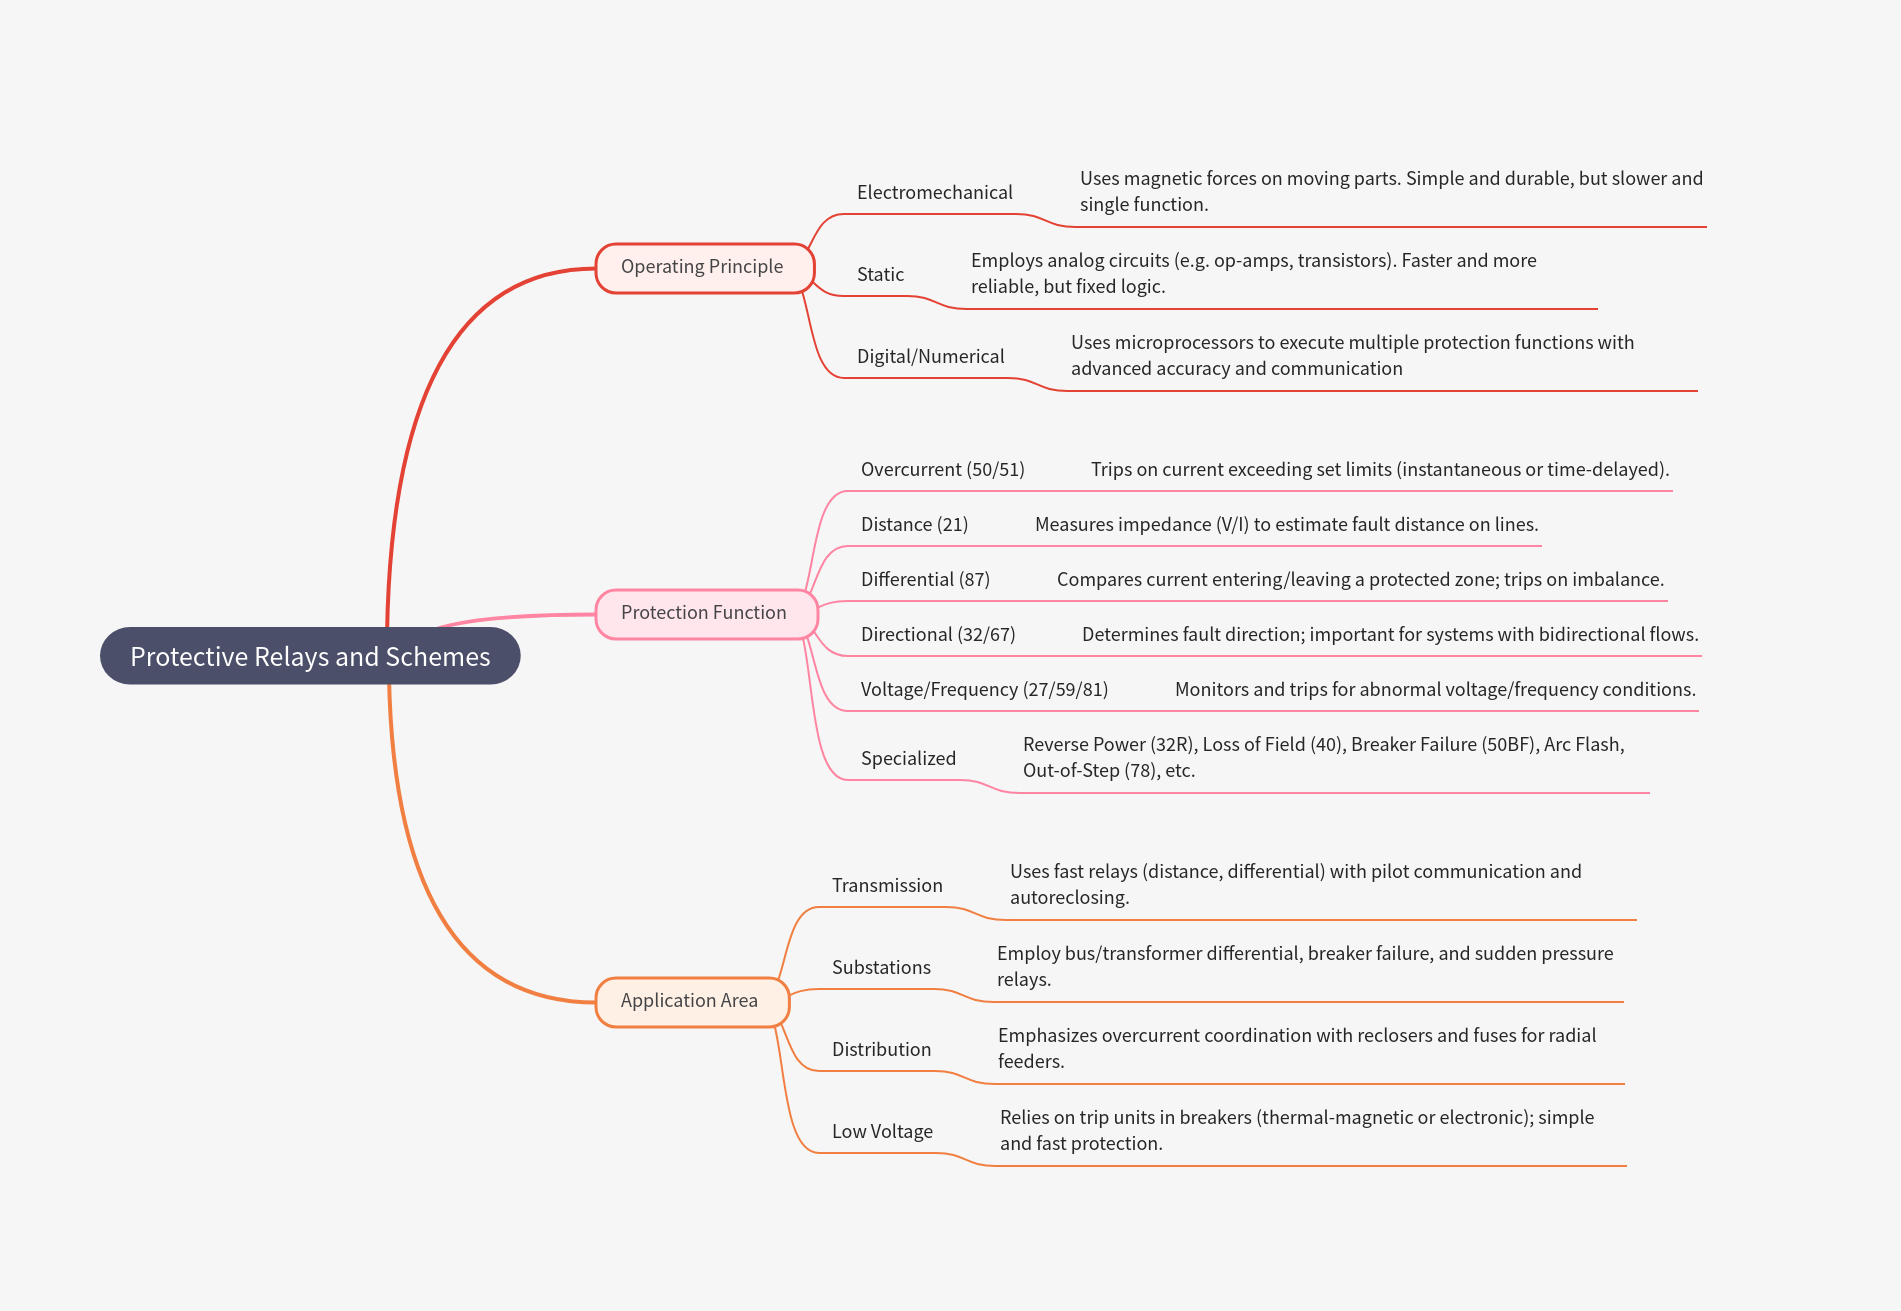
\includegraphics[scale=0.18]{images/chapter_1/ProtectiveRelaysandSchemes.png}
% \caption{Protection relay as a function.}
% \label{Fig:ch_1_vieu}
% \end{figure}






% \subsection{Relay Characteristics}

% Relay operating characteristics—such as inverse-time, definite-time, or directional sensitivity—are chosen based on system topology and coordination needs. Numerical relays allow customizable characteristics (IEC 60255, IEEE C37 standards), adaptive settings, and event-driven reconfiguration, improving dependability in dynamic networks.

% Conventional power system protection schemes perform best when the conditions requiring protection are distinctly different from normal operating conditions. However, they exhibit limitations in certain situations, either failing to provide sufficient protection or struggling to achieve the desired balance between dependability and security. These Some schemes, such as out-of-step and system integrity protection, are optimized for static topologies and may struggle to maintain dependability and security in dynamic systems.
% On the other hand, designing some protection schemes for dynamic or complex power systems is a combination of science and art. This means that there may not be any “standard” designs for such protection challenges. Solutions by different engineers could be different from each other, which can result in differences among the power systems where they are applied and/or the differences in personal experience and knowledge among the designers. In protection coordination studies the major challenge when protection settings are calculated and verified is to achieve settings that are reliable for most operating scenarios of the power system (optimal settings). Power system expansion, new dynamics of equipment, and maintenance constantly add more complexity for finding the optimal settings of protection systems.



% %\subsection{Protection zones and coordination}

% \section{Traditional Power System Protection}


% %\subsection{Traditional Line Protection Relaying}
% % Distance and directional overcurrent protection schemes are widely used in transmission line protection relaying. In this section a background discussion on polarized distance and negative or zero sequence polarized directional overcurrent relays will help to understand how low-magnitude short circuit current with dynamically changing internal impedance (and angle) of an IBR adversely impacts their reliability.

% Conventional schemes rely on overcurrent coordination, assuming unidirectional and high-magnitude fault currents. With DERs, coordination intervals collapse due to low and variable current contributions.

% \subsection{Distance Relay}

% % Many utilities apply mho or Quad characteristics of distance relays for transmission line protection applications. Self-polarized mho characteristic is used as an example to discuss the influence of IBR on the distance relay. Self-polarized mho characteristic is represented by a circle in the first quadrant of R-X plane and passes through origin as shown in Figure. 

% Distance relays measure apparent impedance $(Z_{app}=V/I)$. Under IBR faults, reactive current injection skews the voltage–current phase angle, leading to overreach or underreach depending on the inverter control mode.

% \begin{figure*}[!h]
% \centering
% 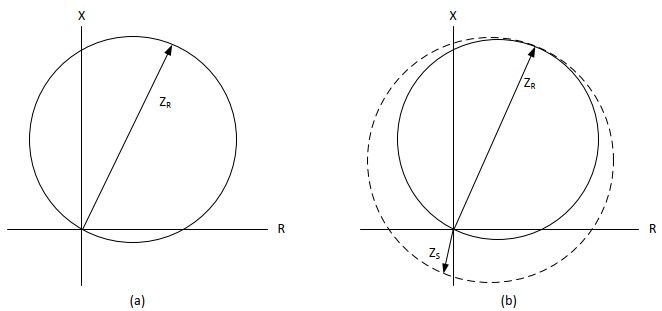
\includegraphics[scale=0.95]{images/chapter_2/Ch2F14Jul.jpg}
% \caption{ Positive sequence Polarized mho distance characteristics (a) without and (b) with dynamic expansion}
% \label{VPP sim}
% \end{figure*}

% \subsection{ Negative or Zero Sequence Polarized Directional Relay}

% % Figure shows an effectively grounded and networked system that has two lines connected in series. These lines tie two systems sourced by traditional synchronous generators. A negative or zero sequence voltage polarized directional relay is shown at Breaker 2 location. This figure has three parts: (a) the top part is a simplified one-line diagram with a solid ground fault in the forward direction of the relay at Breaker 2 location, 
% % (b) negative or zero sequence reactance diagram of the network and (c) 60-Hz phasor diagram illustrating the relationships between negative or zero sequence polarizing voltage and corresponding sequence current for the forward fault seen by the relay at Breaker 2 location. 

% Directional elements using negative- or zero-sequence components face polarity reversals under unbalanced reactive injection. The phase relationship between $(I_2)$ and $(V_2)$ deviates from classical synchronous generator cases, causing misdirection.

% \begin{figure*}[!h]
% \centering
% 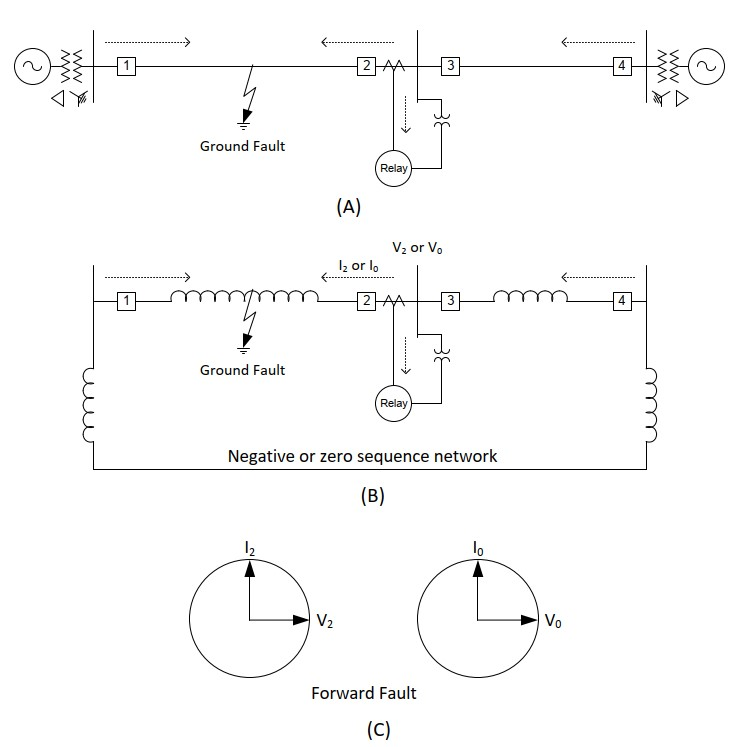
\includegraphics[scale=0.95]{images/chapter_2/Ch2F15Jul.jpg}
% \caption{Negative or zero sequence polarized voltage relationship to its corresponding sequence current for a forward fault with conventional sources at both line terminals}
% \label{VPP sim}
% \end{figure*}

% \begin{figure*}[!h]
% \centering
% 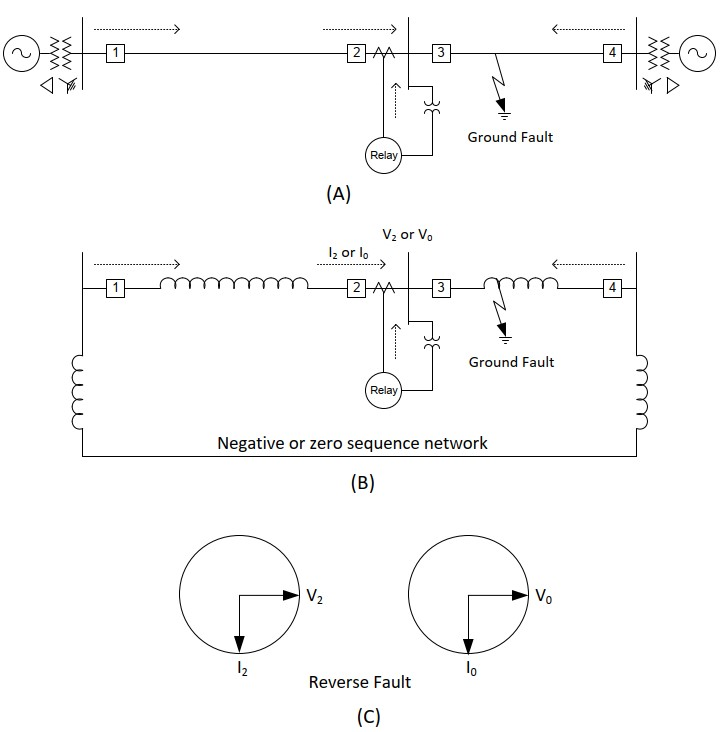
\includegraphics[scale=0.95]{images/chapter_2/Ch2F16Jul.jpg}
% \caption{Negative or zero sequence polarized voltage relationship to its corresponding sequence current for a reverse fault with conventional sources at both line terminals }
% \label{VPP sim}
% \end{figure*}




% \section{Limitations in evolving networks}


% The structural transformation of the modern power system is fundamentally a transition from high-inertia, synchronous-machine-dominated grids to low-inertia, electronically-coupled networks. This shift dismantles the deterministic assumptions of classical protection theory, requiring a rigorous re-evaluation of fault physics and relay response logic.

% \section{Distributed generation (DG) architecture and integration}

% \begin{figure*}[!h]
% \centering
% 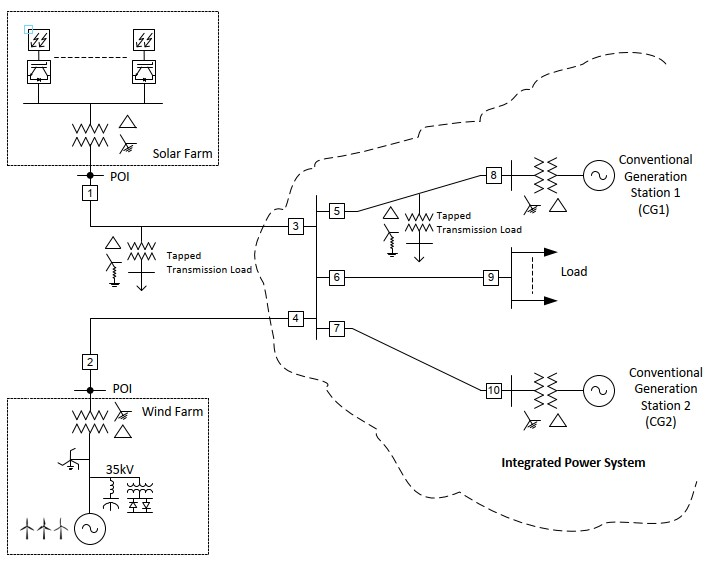
\includegraphics[scale=0.95]{images/chapter_2/Ch2F4Jul.jpg}
% \caption{ Sample interconnection configurations}
% \label{VPP sim}
% \end{figure*}
% Distributed Generation (DG) represents a shift toward decentralized power injection at the distribution or sub-transmission levels. While these resources enhance local voltage profiles and reduce $I^2R$ losses, they transform passive, radial feeders into active, mesh-like networks characterized by bidirectional power flow.

% The protection challenges are primarily dictated by the DG interface technology:

% \begin{itemize}
% \item \textbf{Type I and II :} Employ squirrel-cage (Type I) or wound-rotor (Type II) induction generators. These contribute significant, albeit rapidly decaying, fault currents and lack independent reactive power control.
% \item \textbf{Type III (DFIG) :} Employs a doubly-fed induction generator where the stator is grid-connected and the rotor is interfaced via a partial-scale back-to-back converter. During faults, the "crowbar" protection often activates to protect the converter, temporarily transforming the DFIG into a Type I induction machine with high reactive power consumption.
% \item \textbf{Type IV (Full-Converter) :} These sources, including Solar PV and permanent magnet synchronous generators (PMSG) in wind, are entirely decoupled from the grid frequency via a full-scale DC-link. The fault response is purely a function of control loop parameters and semiconductor thermal limits rather than physical machine constants.
% \end{itemize}

% Each type exhibits distinct dynamic and fault-response behavior, which significantly impacts protection coordination.

% \section{Control of inverter-based resources (grid-following/forming)}

% The integration of Type IV IBRs is governed by the control architecture of the Voltage Source Converter (VSC):

% \begin{itemize}
% \item \textbf{Grid-Following (GFL):} Operates as a high-bandwidth current-controlled source. It utilizes a Phase-Locked Loop (PLL) to track the Point of Common Coupling (PCC) voltage phase angle $\theta$. In weak grids or during severe faults, PLL instability can lead to phase-jumping or loss of synchronism, complicating the relay's phasor estimation.
% \item \textbf{Grid-Forming (GFM) :} Acts as a voltage source, typically employing "droop control" or "virtual synchronous machine" (VSM) algorithms to emulate inertia. GFM inverters provide a reference frequency and voltage, making them the cornerstone of stable islanded microgrid operation.
% \end{itemize}

% \section{Grid Code Requirements}
% Stringent standards like IEEE 1547 and PRC-024-2 have evolved from "disconnect on fault" to "support the grid."
% \begin{itemize}
% \item \textbf{Low-Voltage Ride-Through (LVRT):} Mandates that DGs remain transiently stable during voltage dips, often defined by a $V-t$ characteristic.
% \item \textbf{Dynamic Voltage Support:} Inverters must inject reactive current ($I_q$) in proportion to the voltage drop ($\Delta V$), as governed by a $K$-factor. This injection shifts the current's phase angle, directly impacting the directional sensitivity and impedance calculation of protective relays.
% \end{itemize}

% \section{Fault current behaviour in inverter-dominated systems}
% In synchronous systems, the fault current is characterized by a high sub-transient peak followed by a decay governed by the machine’s time constants ($T''_d$, $T'_d$). Conversely, IBR fault current is:

% \begin{itemize}
% \item \textbf{Magnitude Limited:}  Capped at $1.1\text{--}1.5$ p.u. to prevent IGBT thermal runaway.
% \item \textbf{Controller-Driven:} The current waveform is shaped by the Inner Current Control Loop (ICCL). If the controller uses "Hard Clipping," the resulting current is non-sinusoidal, introducing high-order harmonics that distort Fourier-based phasor estimation in numerical relays.
% \item \textbf{Sequence Component Deficiency:} GFL inverters are often programmed to suppress negative-sequence currents ($I_2$) to protect the DC-link, effectively "blinding" sequence-based fault detection elements.
% \end{itemize}

% \section{Effects on conventional relays}
% The integration of DGs introduces several technical failure modes for legacy protection:
% \begin{itemize}
% \item \textbf{Relay Blinding:} In-feed from DGs increases the voltage at the relay bus while the fault current contribution from the upstream utility remains suppressed, leading to a massive "under-reach" in distance ($21$) and overcurrent ($51$) elements.
% \item \textbf{Sympathetic Tripping:} High DG penetration on a healthy feeder can contribute enough current to a fault on an adjacent feeder to exceed the pickup threshold of its own non-directional relay.
% \item \textbf{Phase Angle Distortion:} $I_q$ injection during LVRT causes the apparent impedance $Z_{app}$ to rotate in the $R-X$ plane, potentially moving the fault trajectory out of the Mho characteristic trip zone.
% \end{itemize}


% \section{Summary of protection issues}
% The overarching conflict is the mismatch between protection sensitivity and system security. In islanded microgrids, the fault current may be lower than the maximum load current in grid-connected mode, rendering static pickup settings mathematically impossible to coordinate without sophisticated adaptive logic.

% \section{Power system protection with distributed generating sources}
% To address these non-linearities, modern protection shifts toward:

% \begin{itemize}
% \item \textbf{Adaptive Protection:} Utilizing a Central Controller to re-calculate relay settings via a "Setting Group Switch" based on real-time SCADA or IEC 61850 GOOSE messaging.
% \item \textbf{Directional Comparison Blocking (DCB):} Essential in microgrids to ensure selectivity when fault currents are bidirectional and low-magnitude.
% \end{itemize}

% \section{Existing solutions - Literature review and identified research gaps}
% Research has moved toward signal-processing-based detection:
% \begin{itemize}
% \item \textbf{Traveling Wave (TW) Protection:} Offers sub-cycle speeds and is independent of magnitude, but requires high-frequency sampling (MHz) and is sensitive to noise.
% \item \textbf{Superimposed Quantities:} Analyzing changes in voltage and current ($\Delta V, \Delta I$) rather than absolute values to improve sensitivity to low-level faults.
% \item \textbf{AI/ML Integration:} Using Convolutional Neural Networks (CNNs) to classify faults based on raw time-domain signatures.
% \end{itemize}

% \section{Ranking and gap analysis}
% % Requires: \usepackage{booktabs}
% \begin{table}[h]
%     \centering
%     \caption{Placeholder Caption}
%     \label{tab:placeholder_label}
%     \begin{tabular}{llll}
%         \toprule
%         Protection Method & Speed   & Sensitivity to IBRs & Dependency                  \\
%         \midrule
%         Traditional Overcurrent (51) & Slow    & Very Low            & Fault Magnitude            \\
%         Distance (21)                & Medium  & Low                 & Source Impedance Ratio (SIR) \\
%         Line Differential (87L)      & Fast    & High                & Reliable Communication     \\
%         Adaptive Logic               & Variable & High               & System Topology Data       \\
%         \bottomrule
%     \end{tabular}
% \end{table}

% \section{Problem statement and research gap}
% The primary research gap lies in the autonomous detection of high-impedance faults (HIF) and symmetrical faults in IBR-heavy microgrids without reliance on high-bandwidth communication. Existing literature heavily focuses on either pure communication-based differential schemes or local adaptive methods that fail during "Load Encroachment" scenarios. There is an urgent need for a robust, multi-dimensional protection logic—potentially integrating the Load Blinder (21LB) function with adaptive sequence-current analysis—to distinguish between heavy loads, IBR transients, and genuine low-magnitude faults.


% \section{Protection issues with IBR}

% % This section highlights challenges to traditional protection schemes, such as directional ground fault, negative sequence overcurrent, phase distance, differential and power swing protection when used for protecting lines with IBR.

% IBRs distort current waveforms, limit magnitudes, and change phase angles dynamically, posing major challenges:

% Reduced sensitivity of overcurrent protection.

% Incorrect reach of impedance relays.

% Reverse directional tripping under LVRT support.

% \subsection{ Negative Sequence Based Directional Ground Fault Relaying}

% In conventional systems, ground fault direction is determined from the phase of (I_2) relative to (V_2). In IBRs, negative-sequence reactive injection shifts this phase, leading to 90°–180° error. Modified directional logic using instantaneous reactive power polarity or dq-frame reactive component sign has been proposed to mitigate this issue.

% % Example 1: A single phase-to-ground fault evolving to a double phase-to-ground fault supplied by large Type III wind turbine facilities \\
% % Example 2: A single phase-to-ground fault supplied by a large solar generation facility \\
% % Example 3: A single phase-to-ground fault where fault current contribution from Static Synchronous Compensator or STATCOM source contributed to undesirable line protection operation for an out-of-zone fault \\
% % Example 4: A phase-to-phase fault supplied by a Type IV wind turbine generator facility 


% %\section{Microgrid network architecture}

\section{Test system validations using MATLAB/Simulink and PSCAD result}

\subsubsection{ Example 1 – Type III Wind Turbine Generator}

Type III wind turbine generator stators are directly connected to the grid as shown in Figure 3. The generator rotors are built with three-phase windings which receive their excitation from a power converter also connected to the grid. Since the converter system is only interfaced to the rotor circuit and the stator is directly connected to the grid, the power 
converter contributes only partial i.e. 30-40\% of the generator rated power. The laminated rotor with short time flux time constant and power electronic excitation system provides fast reactive power control and voltage regulation. 

\begin{figure*}[!h]
\centering
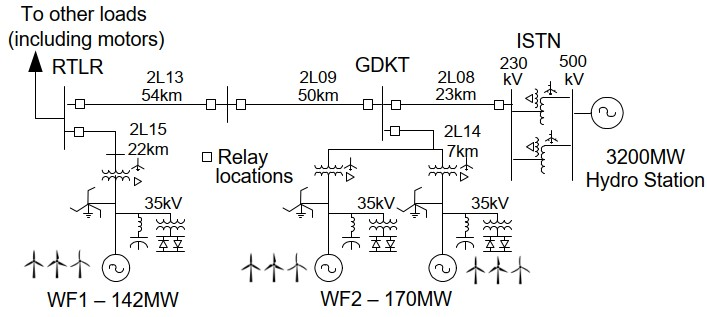
\includegraphics[scale=0.95]{images/chapter_2/Ch2F17Jul.jpg}
\caption{System One-line diagram – Example 1}
\label{VPP sim}
\end{figure*}

Ground Short Circuit Analysis: \\

\begin{figure*}[!h]
\centering
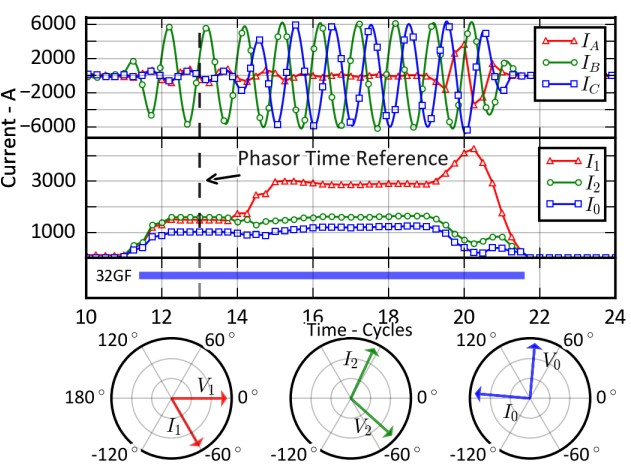
\includegraphics[scale=0.95]{images/chapter_2/Ch2F18Jul.jpg}
\caption{Relay records for an evolving forward ground fault contributed by conventional synchronous source. }
\label{VPP sim}
\end{figure*}

\begin{figure*}[!h]
\centering
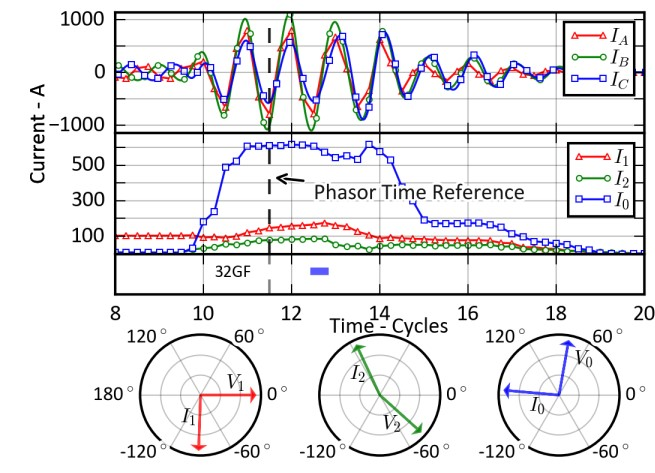
\includegraphics[scale=0.95]{images/chapter_2/Ch2F19Jul.jpg}
\caption{Relay records for an evolving forward ground fault contributed by Type III wind turbine generator}
\label{VPP sim}
\end{figure*}

\begin{figure*}[!h]
\centering
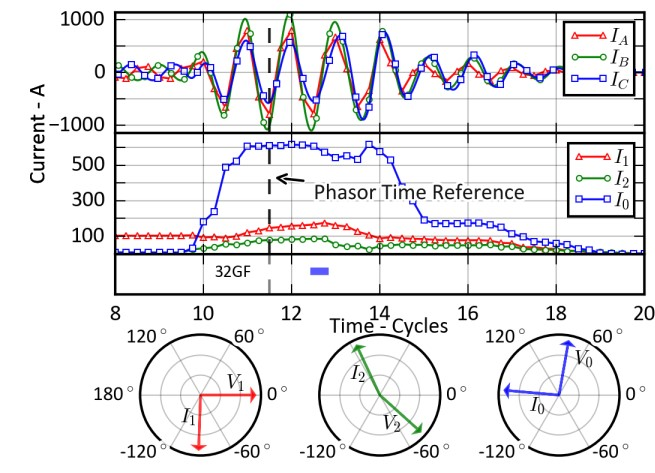
\includegraphics[scale=0.95]{images/chapter_2/Ch2F19Jul.jpg}
\caption{Relay records for an evolving reverse ground fault contributed by Type III wind turbine generator}
\label{VPP sim}
\end{figure*}

Short circuit current analysis confirmed that the negative sequence current phase angle relationship with the negative sequence voltage from a Type III wind turbine generator is unlike that of conventional synchronous sources and is not readily known. Therefore, a conventional negative sequence current based scheme can’t provide reliable directional protection against ground faults in situations with high penetrations of IBR influencing short circuit currents. However, if these generators are connected through a transformer that is a source of zero sequence current, then ground fault protection can be achieved using zero sequence current. The protection will be predominantly independent of the type of wind turbine generator or its associated control algorithm because the interconnecting transformer, not wind the turbine generation, is the source of zero sequence current. 



\subsubsection{Example 2 – Solar Generation Facility}

A solar (photovoltaics) generation facility interconnects to the grid through a DC-AC inverter system. Typically the fault current from the inverter is governed by the inverter control system within two cycles after the short circuit. In the absence of an interconnection or grid code requirement, the control system is often programmed to restrict the magnitude of negative sequence current. If an inverter design permits limited supply of negative sequence current, it may have non-inductive source characteristic angle rendering unreliable in decisions from the devices operating on negative sequence relaying principles. This section compares line-to-ground short circuits from strong utility sources and solar resources to illustrate that negative sequence relaying cannot be applied on a line connecting a solar facility producing negative sequence in insufficient magnitude and/or phase angle.

\begin{figure*}[!h]
\centering
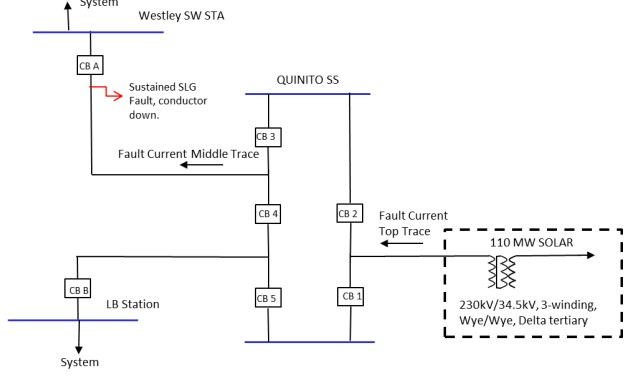
\includegraphics[scale=0.95]{images/chapter_2/Ch2F21Jul.jpg}
\caption{System One-line diagram – Example 2}
\label{VPP sim}
\end{figure*}

Ground Short Circuit Analysis: \\

\begin{figure*}[!h]
\centering
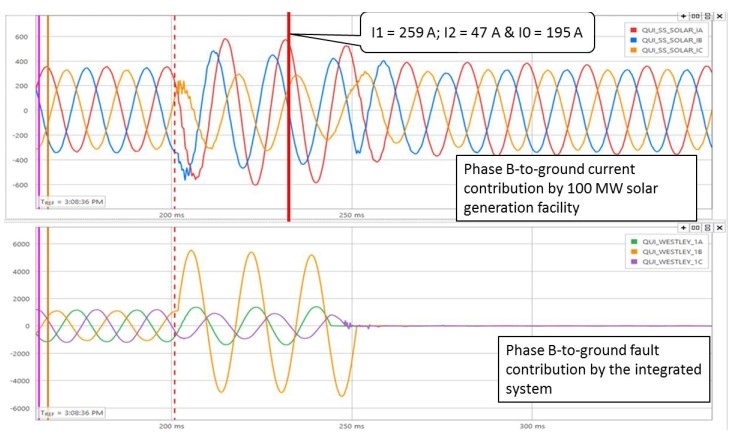
\includegraphics[scale=0.95]{images/chapter_2/Ch2F22Jul.jpg}
\caption{Relay records for a single phase-to-ground fault contributed by the solar generation facility and integrated system }
\label{VPP sim}
\end{figure*}

In the absence of an interconnection grid code, the inverter control system of solar generation facility will likely restrict the magnitude of negative sequence current during unbalanced faults. As a consequence, the negative sequence relaying cannot be reliably applied on a line connecting a solar facility with this characteristic.





\subsubsection{Example 4 – Type IV Wind Turbine Generator }


This section describes a simulation based study performed to demonstrate an example of negative sequence directional relay misoperation on short circuit current response of a 300 MW Type IV wind turbine generator facility during a phase-to-phase fault. This facility is comprised of 200×1.5 MW Type IV wind turbine generators whose control system completely suppresses negative sequence current. 

\begin{figure*}[!h]
\centering
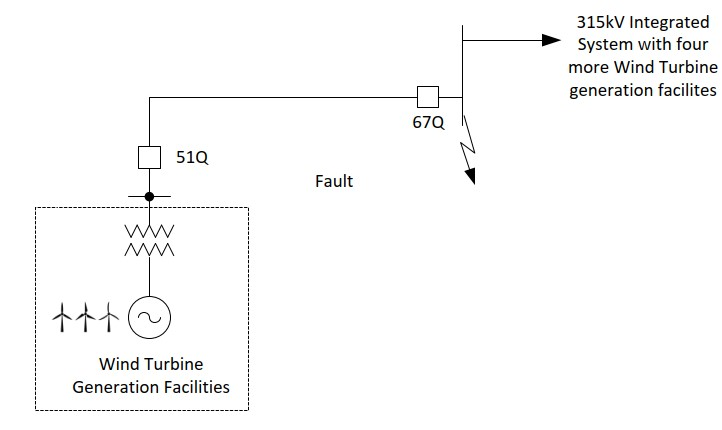
\includegraphics[scale=0.95]{images/chapter_2/Ch2F27Jul.jpg}
\caption{SSystem One-line diagram – Example 4}
\label{VPP sim}
\end{figure*}

Scenario 1: The wind facility as shown in the figure was replaced with a synchronous generator of equal (300 MVA) capacity \\
Scenario 2: The original facility comprising of 200×1.5 MW Type IV wind turbine generators coupled sequence control (CSC) scheme, i.e. with no negative current injection control capability\\ 
Scenario 3: The wind facility comprising of 200×1.5 MW Type IV wind turbine generators decoupled sequence control (DSC) scheme [10], i.e. with negative sequence current injection control capability similar to Figure 8 

Simulated Phase-to-Phase Analysis: \\

\begin{figure*}[!h]
\centering
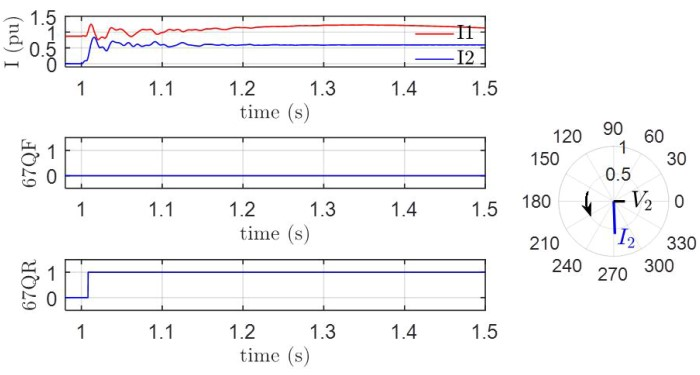
\includegraphics[scale=0.95]{images/chapter_2/Ch2F28Jul.jpg}
\caption{Negative sequence voltage polarized relay responses to simulated phase-to-phase fault with synchronous generator – Scenario 1}
\label{VPP sim}
\end{figure*}

\begin{figure*}[!h]
\centering
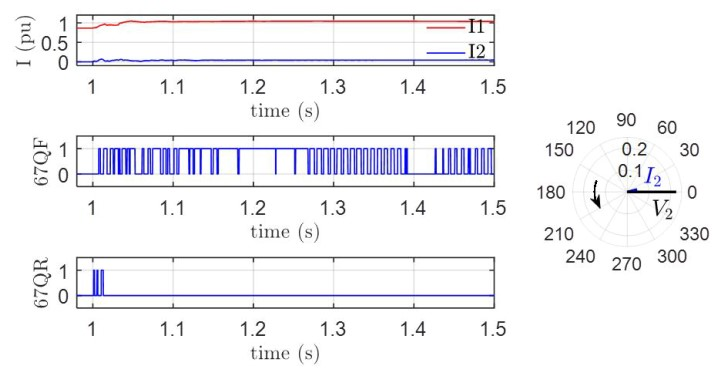
\includegraphics[scale=0.95]{images/chapter_2/Ch2F29Jul.jpg}
\caption{Negative sequence voltage polarized relay responses to simulated phase-to-phase fault with coupled controlled (no negative sequence current injection capability) Type IV wind turbine generators – Scenario 2 }
\label{VPP sim}
\end{figure*}

\begin{figure*}[!h]
\centering
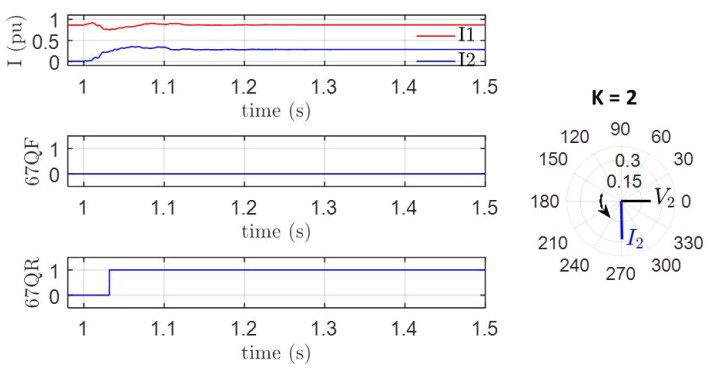
\includegraphics[scale=0.95]{images/chapter_2/Ch2F30Jul.jpg}
\caption{Negative sequence voltage polarized relay responses to simulated phase-to-phase fault with decoupled controlled negative sequence current injection capability and K=2) Type IV wind turbine generators – Scenario 3 }
\label{VPP sim}
\end{figure*}

Type IV wind turbine generation exhibits a substantially different negative-sequence fault current characteristic compared to synchronous generators. IBR without negative sequence injection capability may negatively impact the performance of negative-sequence directional relay element due to the changed angular relation of negative sequence quantities. 
All relaying devices require minimum (settable or non-settable threshold) negative sequence current to maximize reliability of their directional decisions. In the absence of negative sequence current i.e. when it is below minimum threshold, relay behavior can vary from either blocking directional element or converting the directional to non-directional element.  

\subsection{Negative Sequence Overcurrent Relaying}

This section presents the following two examples, field and simulated events, demonstrating that traditional negative sequence overcurrent unreliability when operating on short current supplied by the IBR facilities: \\
Example 1:An event involving phase-to-phase-to-ground fault sourced by battery storage and inverter system \\
Example 2:An event involving phase-to-phase fault supplied by Type III or IV wind turbine generator 

\subsubsection{Example 1}

Photovoltaic or battery storage systems are DC sources that connect to grid through an inverter interface. In absence of grid code, most inverters are programmed to balance their terminal voltage and to suppress their negative sequence current output. Thus, their apparent negative sequence source impedance is typically significantly higher than their positive sequence source impedance. On fault inception, they respond to voltage drop and increase their positive sequence current to a pre-specified current threshold i.e. at their thermal rating. At this level, the inverter almost acts as a current source until the voltage recovers. This section illustrates that the negative sequence protection cannot be reliably applied when the relay operating current is solely supplied by the IBR. Though the example used is from the distribution system, the lessons learned from this application apply to transmission connected IBR as well.

\begin{figure*}[!h]
\centering
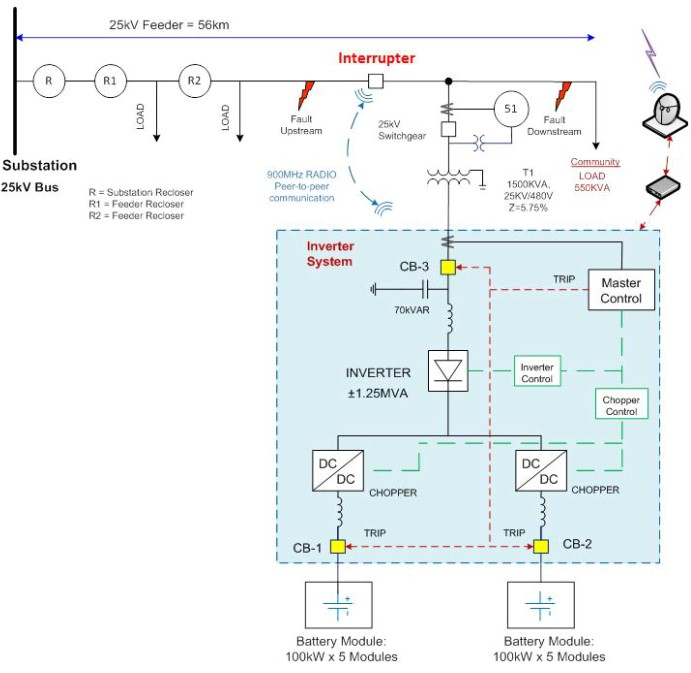
\includegraphics[scale=0.95]{images/chapter_2/Ch2F31Jul.jpg}
\caption{Electrical one-line diagram showing interconnection of DC battery and inverter system  }
\label{VPP sim}
\end{figure*}


\begin{figure*}[!h]
\centering
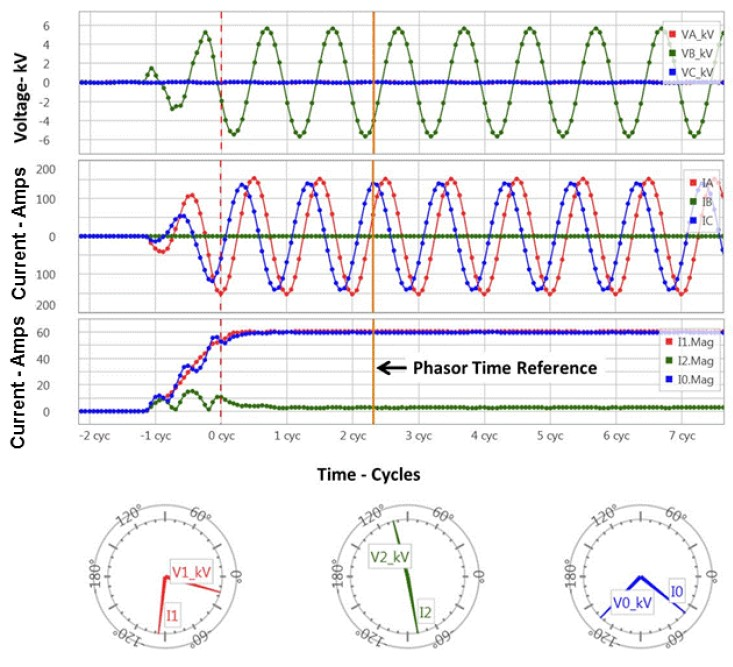
\includegraphics[scale=0.95]{images/chapter_2/Ch2F32Jul.jpg}
\caption{Inverter system response to line-to-line-to-ground fault}
\label{VPP sim}
\end{figure*}

Short circuit current analysis of the recorded ground fault confirmed that the negative sequence source impedance of the inverter source can be significantly high. Thus, negative sequence current can be too small to use in reliable relaying decisions. Inverter systems are typically ungrounded but they typically connect through an interconnection transformer that provides effective grounding to the high voltage network. As seen in previous examples, the reliability of zero sequence relaying largely remains unhindered by high penetration of inverter sources as long as these sources are connected using a transformer which provides a path for zero sequence current. 



\subsubsection{Example 2 – Simulated Event}

This section presents a simulation study of an actual system demonstrating challenges when applying a negative sequence overcurrent relay to the fault current contribution from Type III and Type IV wind turbine generation facilities.


 Simulated Phase-to-Phase Analysis: 
A permanent phase-to-phase fault, as shown in Figure 27, was simulated. It was applied at t=1.0 s on the line interconnecting the 200×1.5 MW wind turbine facility to the rest of the grid. A negative sequence inverse-time overcurrent relay, denoted by 51Q, is assumed, on the line terminal leaving the wind generation facility. The primary negative sequence overcurrent (I2) pickup was set at 330 A which was about 0.6 pu of the facility rated output. The following three scenarios were simulated to illustrate challenges of applying negative sequence overcurrent protection on a line terminal connected to the IBR facility. \\
Scenario 1: The wind facility as shown in Figure was replaced with a synchronous generators of equal (300 MVA) capacity \\
Scenario 2: The original facility comprising of 200×1.5 MW Type IV wind turbine generators  \\
Scenario 3: The original facility comprising of 200×1.5 MW Type III wind turbine generators \\

\begin{figure*}[!h]
\centering
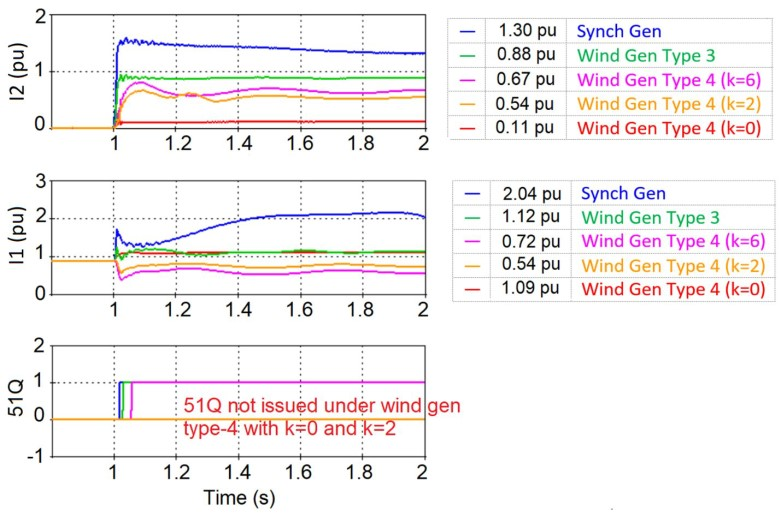
\includegraphics[scale=0.95]{images/chapter_2/Ch2F33Jul.jpg}
\caption{Negative and positive sequence currents along with statuses of 51Q for a phase-to-phase fault with different resources}
\label{VPP sim}
\end{figure*}

Depending upon the pick-up setting, this study illustrates that negative sequence overcurrent relaying poses a dependability risk for transmission lines connecting to Type IV wind generator facility whose control system has a low negative sequence current gain (k) injection setting. Type III generators supply some negative sequence current which is much smaller than the conventional synchronous generator for the same fault. Thus 
inverse-time coordination with the negative sequence overcurrent relays, where there is high penetration of Type III wind turbine generation, can be challenging without detailed understanding of each facility control system. 

\subsection{Phase Distance Relaying}


Following is an example where the line distance relay failed to operate on a fault internal to the line protection zone as well as could not provide backup for the external fault. The failure was largely attributed to a specific control mode setting of the IBR facility and the protection application engineers may not have been familiar with this operating mode. 

\begin{figure*}[!h]
\centering
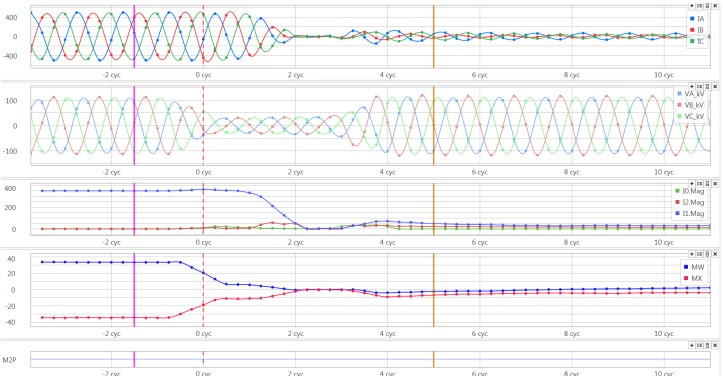
\includegraphics[scale=0.95]{images/chapter_2/Ch2F34Jul.jpg}
\caption{Three-phase short circuit response of a Type IV wind turbine generator operating in ZPM }
\label{VPP sim}
\end{figure*}

\begin{figure*}[!h]
\centering
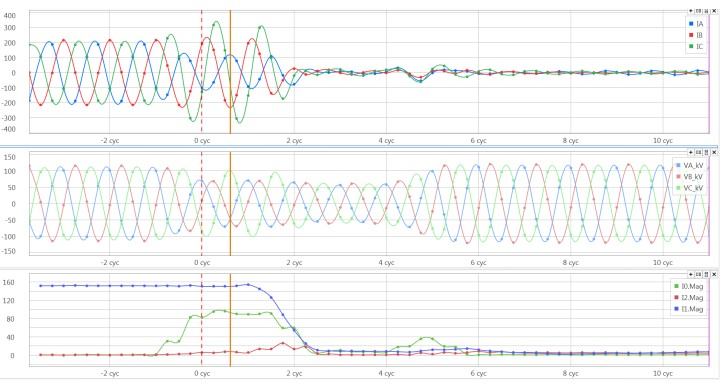
\includegraphics[scale=0.95]{images/chapter_2/Ch2F35Jul.jpg}
\caption{Data recorded by 138 kV line relay showing response of an IBR to an 
external unbalanced fault}
\label{VPP sim}
\end{figure*}


ZPM suspends the output current within two cycles of voltage depression when the IBR facility is still connected to the line. While this mode allows the IBR to ride through voltage depressions (low voltage ride through) during external faults, it also inhibits the distance (or overcurrent) protection for the internal line faults. Prevalent deployment of ZPM operation in the existing IBR facilities and its risk to the system, particularly to raditional line protection, reliability was not well known until 
recently. On 16 August, 2016, the Blue Cut Fire in California caused a 500kV line fault. Though the fault was cleared in less than 3 cycles, pproximately 1200 MW of solar generation was coincidently either temporarily suspended or lost. Subsequent investigation by the NERC/WECC joint task force reported  that the majority of lost solar generation was caused by the zero operational mode i.e. IBR were configured to momentarily cease 
current injection for voltages outside their continuous operating range. 

% \section{Challenges to System Protection Schemes and Solutions}

% The control system of a radially connected IBR (particularly Type III wind turbine generator) facility to a series capacitor compensated  line can excite undamped and damaging subsynchronous oscillations. Unintentional IBR  islanding can subject the customer loads in the island to poor power quality with damaging  consequences. This section discusses these new challenges and methods to address them.

% IBRs introduce low inertia, dynamic reactance, and voltage-dependent current control, breaking conventional assumptions of protection design. Potential solutions include:

% Adaptive relays using synchrophasor and digital twin feedback.

% Voltage-based and reactive power directional protection (EVPM).

% AI/ML classifiers distinguishing LVRT from genuine faults.

% Communication-assisted wide-area coordination.

% \subsection{Power Swing Protection Schemes}

% % Since IBR have no inherent rotational inertia, power swing characteristics may be substantially different than that under synchronous generation. Such different swing characteristics may result in the misoperation of a legacy power swing protection system.

% IBRs modify system power–angle stability, reducing natural damping. Hence, distance relay power swing blocking (PSB) must distinguish between true swings and voltage-controlled inverter oscillations. Hybrid impedance–energy-based criteria are emerging to handle these scenarios.

% \subsubsection{PSB Misoperation due to IBR }

% A three-phase fault with a time duration of 270 ms was applied on line L2 close to Substation E followed by the outage of lines L2 and L4 at t = 2 s resulting in an out-of-step condition. The event was simulated under 0\% and 25\% IBR penetration levels realized by replacing Generator G1 with a Type III or Type IV wind turbine or solar PV generator (W1). However results from simulation of Type III wind turbine generator are presented in this section because they were similar for Type IV wind turbine and solar PV generator, 
% assuming the same inverter controls. Figure 38 depicts the swing impedance trajectory during the first 30 cycles of the power swing, and Figure 39 shows the response of distance and power swing elements. As shown under 0\% wind turbine generation, the impedance trajectory crossed the outer and middle elements in more than the PSB time delay setting of three cycles (48 ms). Hence, the PSB successfully detected the swing and issued a PSB signal to block all tripping zones of distance protection elements. Under 25\% wind turbine generation, the impedance trajectory crossed the outer and middle elements in less than the PSB time delay setting. Hence, the power swing protection failed to detect the power swing and did not issue the PSB signal. As the swing continued, the impedance trajectory entered Zone 2, and the power swing was mistakenly declared as a fault in Zone 2 which was picked up by the distance protection. This could result in undesired tripping of line L1
% \begin{figure*}[!h]
% \centering
% 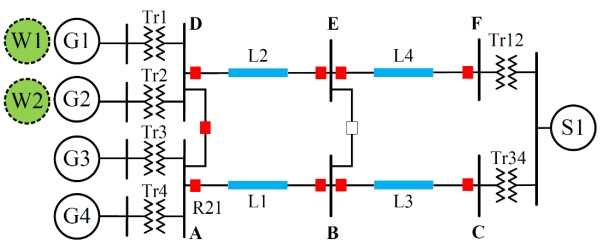
\includegraphics[scale=0.95]{images/chapter_2/Ch2F37Jul.jpg}
% \caption{IEEE PSRC WG-D6 test system including wind generation}
% \label{VPP sim}
% \end{figure*}

% \begin{figure*}[!h]
% \centering
% 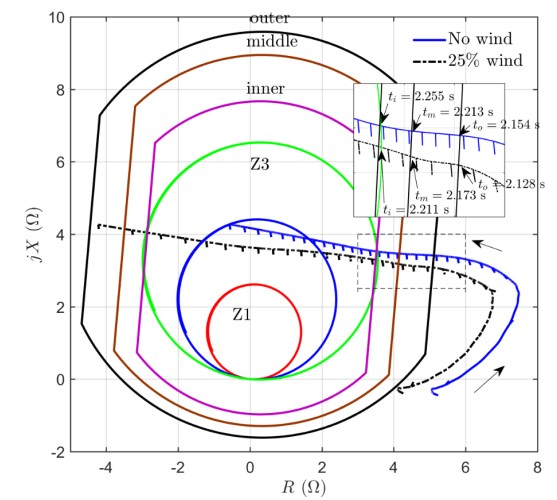
\includegraphics[scale=0.95]{images/chapter_2/Ch2F38Jul.jpg}
% \caption{Swing impedance trajectory under 0\% (blue) and 25\% wind generation 
% (dashed black)}
% \label{VPP sim}
% \end{figure*}

% \begin{figure*}[!h]
% \centering
% 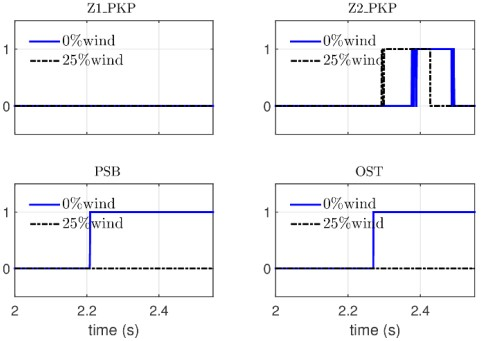
\includegraphics[scale=0.95]{images/chapter_2/Ch2F39Jul.jpg}
% \caption{Distance and power swing relay signals under 0\% (blue) and 25\% wind generation (dashed black))}
% \label{VPP sim}
% \end{figure*}

% \subsubsection{OST Misoperation due to IBR}
% This case study compares the most severe stable swing under 0\% and 50\% IBR levels. In simulations, Synchronous Generators G1 and G2 were replaced with Type III or Type IV wind turbine or solar PV generators (W1 and W2). The simulations shown in this section were conducted with Type III wind turbine generator models, however similar results were observed with Type IV wind turbine and solar PV generators, assuming the same inverter controls. 
% Under 0\% wind, the most severe stable swing was caused by an 88 ms three-phase fault on line L2 close to substation E followed by the outage of lines L2 and L4. But under 50\% wind generation, the most severe stable swing was caused by 120 ms fault. Figure 40 depicts the swing impedance trajectory of the most severe stable swing under 0\% and 50\% wind generation, and Figure 41 shows the response of power swing protection.

% \begin{figure*}[!h]
% \centering
% 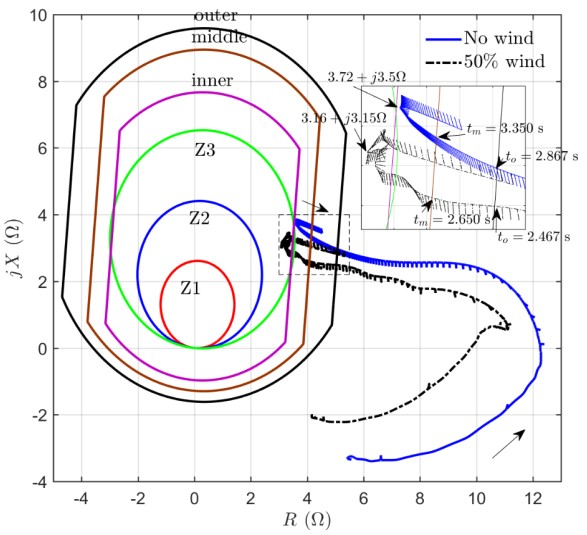
\includegraphics[scale=0.95]{images/chapter_2/Ch2F40Jul.jpg}
% \caption{Swing impedance trajectory of the most severe stable swing under 0\% (blue) and 50\% wind generation (dashed black)}
% \label{VPP sim}
% \end{figure*}

% \begin{figure*}[!h]
% \centering
% 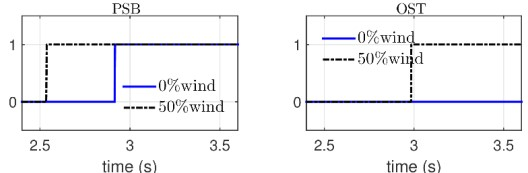
\includegraphics[scale=0.95]{images/chapter_2/Ch2F41Jul.jpg}
% \caption{Power swing relay signals under 0\% (blue) and 50\% wind generation (dashed black)}
% \label{VPP sim}
% \end{figure*}

% \section{IBR Islanding Considerations }


% Anti-islanding schemes continue to evolve with technology and algorithm advancements within inverter controls. Historically the transmission owner was responsible for disconnecting non-utility generation connected to transmission system during an islanding event. Modern inverters may have built-in active and passive anti-islanding controls that will shut down the source in an islanding event. As with most protection challenges Selecting the best anti-islanding scheme requires a delicate balance between aintaining
% acceptable levels of power quality, maintaining minimum voltage and requency ride through support during transient events, and cost. 


% \subsection{Anti-Islanding Guides and NERC Standards} 

% % Inverters may have built-in passive and/or active anti-islanding detection systems. Passive anti-islanding detection methods are based on a (passive) measurement of the grid values. Active method means that the inverter makes something active and gets back a reaction of the grid. This reaction is very different in case of islanding grid, compared with normal grid operation. Inverters may use voltage and frequency measurements as passive islanding 
% % methods, and employ the escalating frequency shift method as an active detection system. The IEEE standard 1547-2018 applies mainly to distribution connected resources. For an unintentional island in which the distribution resource energizes a portion of the Area Electric Power System (EPS) through POI, the distribution resource shall detect the island, cease to energize the Area EPS, and trip within 2 seconds of the formation of an island. The anti-islanding scheme must be secure enough to not operate under false 
% % conditions. 

% Islanding occurs when a portion of the network continues energized by DERs after grid disconnection. IEEE 1547 and NERC PRC-024 require detection within 2 seconds using:

% Passive methods (ROCOF, voltage phase jump).

% Active methods (impedance injection).
% However, these become less effective as IBR penetration increases, demanding hybrid adaptive detection using real-time system identification or AI.



% % \section{Modelling Wind Sources}

% % \begin{figure*}[!h]
% % \centering
% % 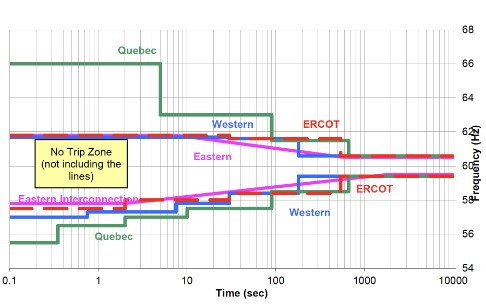
\includegraphics[scale=0.95]{images/chapter_2/Ch2F4.jpg}
% % \caption{FRT requirements}
% % \label{VPP sim}
% % \end{figure*}

% % \begin{figure*}[!h]
% % \centering
% % 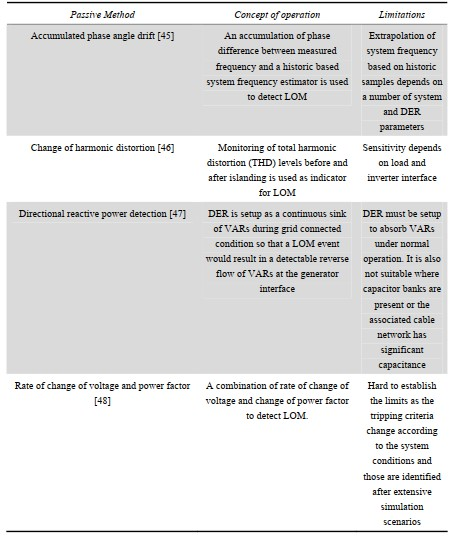
\includegraphics[scale=0.95]{images/chapter_2/Ch2F5.jpg}
% % \caption{Passive methods for improved LOM protection}
% % \label{VPP sim}
% % \end{figure*}


% % \begin{figure*}[!h]
% % \centering
% % 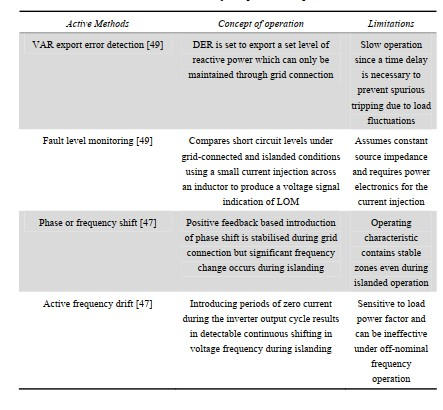
\includegraphics[scale=0.95]{images/chapter_2/Ch2F6.jpg}
% % \caption{Active methods for improved LOM protection}
% % \label{VPP sim}
% % \end{figure*}

% % \begin{figure*}[!h]
% % \centering
% % 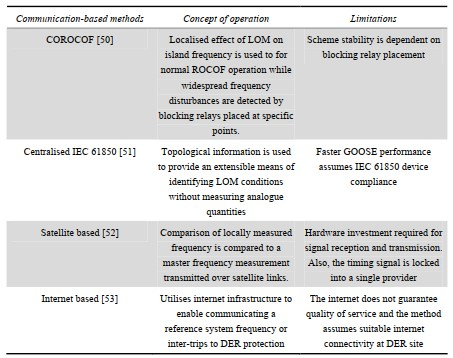
\includegraphics[scale=0.95]{images/chapter_2/Ch2F7.jpg}
% % \caption{Communications based methods for improved LOM protection }
% % \label{VPP sim}
% % \end{figure*}


% % \section{Protection issues with DERs}

% % \begin{figure*}[!h]
% % \centering
% % 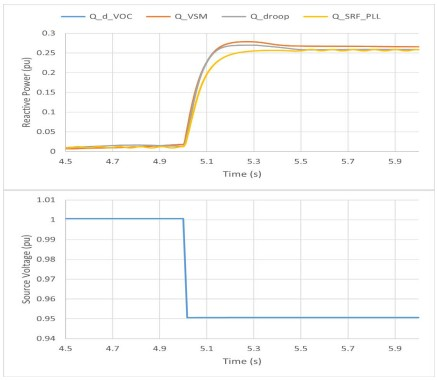
\includegraphics[scale=0.95]{images/chapter_2/Ch2Graph1.jpg}
% % \caption{Generic GFM model output for a step decrease in source voltage at t = 5 s}
% % \label{VPP sim}
% % \end{figure*}

% % \begin{figure*}[!h]
% % \centering
% % 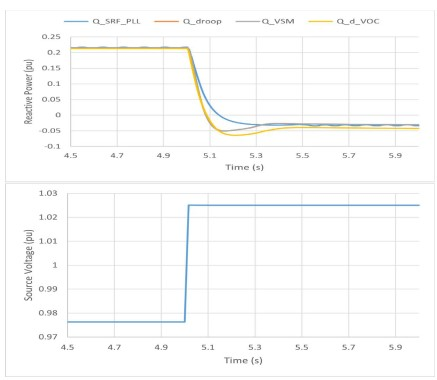
\includegraphics[scale=0.95]{images/chapter_2/Ch2Graph2.jpg}
% % \caption{Generic GFM model output for a step decrease in source voltage at t = 5 s}
% % \label{VPP sim}
% % \end{figure*}

% % \begin{figure*}[!h]
% % \centering
% % 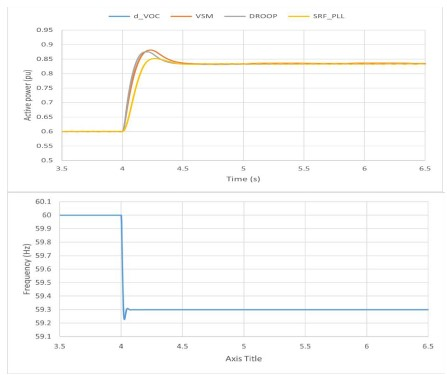
\includegraphics[scale=0.95]{images/chapter_2/Ch2Graph3.jpg}
% % \caption{Generic GFM model output for a step decrease in source voltage at t = 5 s}
% % \label{VPP sim}
% % \end{figure*}

% % \begin{figure*}[!h]
% % \centering
% % 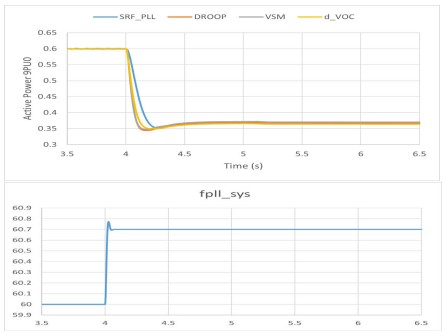
\includegraphics[scale=0.95]{images/chapter_2/Ch2Graph4.jpg}
% % \caption{Generic GFM model output for a step decrease in source voltage at t = 5 s}
% % \label{VPP sim}
% % \end{figure*}
% % Apparent impedance measured by distance relay
% \begin{equation}
% \label{eq:zapp}
% Z_{app} = \frac{V_{ph}}{I_{ph}}
% \end{equation}

% % Instantaneous active and reactive power
% \begin{equation}
% \label{eq:pq}
% \begin{aligned}
% p(t) &= v_\alpha i_\alpha + v_\beta i_\beta \\
% q(t) &= v_\beta i_\alpha - v_\alpha i_\beta
% \end{aligned}
% \end{equation}

% % dq-domain power expressions
% \begin{equation}
% \label{eq:pq_dq}
% \begin{aligned}
% P &= \frac{3}{2}(v_d i_d + v_q i_q) \\
% Q &= \frac{3}{2}(v_q i_d - v_d i_q)
% \end{aligned}
% \end{equation}

% % PLL angle estimation
% \begin{equation}
% \label{eq:pll}
% \theta_{PLL}(t) = \int_0^t \omega_{PLL}(\tau) \, d\tau
% \end{equation}

% % Active power-frequency droop for FRT
% \begin{equation}
% \label{eq:droop}
% \Delta P = K_f (\omega_{ref} - \omega)
% \end{equation}

% % Inverter current response to voltage sag (control loop dynamics)
% \begin{equation}
% \label{eq:curr_dyn}
% L \frac{d\mathbf{I_{dq}}}{dt} = \mathbf{V_{conv,dq}} - \mathbf{V_{pcc,dq}} - R\mathbf{I_{dq}}
% \end{equation}

% % Symmetrical component transformation
% \begin{equation}
% \label{eq:sym_comp}
% \begin{bmatrix}
% I_0 \\ I_1 \\ I_2
% \end{bmatrix}
% = \frac{1}{3}
% \begin{bmatrix}
% 1 & 1 & 1 \\
% 1 & a & a^2 \\
% 1 & a^2 & a
% \end{bmatrix}
% \begin{bmatrix}
% I_a \\ I_b \\ I_c
% \end{bmatrix}
% \end{equation}
% where $a = e^{j120^\circ}$

% % Fault current contribution of inverter (controlled current source)
% \begin{equation}
% \label{eq:ifault}
% \mathbf{I_{fault}} = I_{max} e^{j\phi_c}
% \end{equation}
% where $\phi_c$ is the control-defined phase angle of the injected current.

% % Negative sequence directional element torque equation
% \begin{equation}
% \label{eq:dir_torque}
% T_{d2} = |V_2||I_2|\cos(\theta_{V2} - \theta_{I2} - \delta)
% \end{equation}

% % Apparent impedance trajectory due to reactive current injection
% \begin{equation}
% \label{eq:ztraj}
% Z_{app}(t) = \frac{V_{pref} - \Delta V(t)}{I_{pref} + \Delta I_q(t)}
% \end{equation}

% % Voltage support under LVRT control
% \begin{equation}
% \label{eq:v_support}
% V_{pcc}(t) = V_{pre} + \frac{X_{eq}}{V_{base}} I_q(t)
% \end{equation}

% % Power electronic converter energy balance
% \begin{equation}
% \label{eq:energy_dc}
% C_{dc}\frac{dV_{dc}}{dt} = I_{pv} - I_{conv}
% \end{equation}

% % Grid-side converter active and reactive power exchange
% \begin{equation}
% \label{eq:pq_grid}
% \begin{aligned}
% P_{grid} &= \frac{3}{2}V_d I_d \\
% Q_{grid} &= -\frac{3}{2}V_d I_q
% \end{aligned}
% \end{equation}

% % Phase voltage under unbalanced fault condition
% \begin{equation}
% \label{eq:vphase}
% V_a = V_1 + V_2 + V_0
% \end{equation}

% % DER protection threshold adaptive setting
% \begin{equation}
% \label{eq:adaptive}
% I_{set}(t) = I_{base} + k_\Delta \frac{dV_{pcc}}{dt}
% \end{equation}

% % Equivalent circuit impedance of converter under short circuit
% \begin{equation}
% \label{eq:zeq}
% Z_{eq} = R_f + j(\omega L_f + X_c)
% \end{equation}

% % Frequency ride through droop control
% \begin{equation}
% \label{eq:frt}
% P(t) = P_{nom}\left[1 + K_p(\omega - \omega_{ref})\right]
% \end{equation}

% % Reactive current injection under voltage unbalance
% \begin{equation}
% \label{eq:iq_inj}
% I_q = K_{pos}(1 - V_1/V_{nom}) + K_{neg}(V_2/V_{nom})
% \end{equation}

% % Directional decision using reactive power polarity (EVPM concept)
% \begin{equation}
% \label{eq:evpm}
% Q_{inst} = v_\alpha i_\beta - v_\beta i_\alpha
% \end{equation}
% If $Q_{inst} > 0$, the fault is in the forward direction; else, reverse.



% \section{Conclusion}
% This chapter examined short-circuit modeling of IBRs and their implications for conventional protection. It demonstrated that IBRs behave as controlled current sources governed by converter and grid code logic, significantly altering fault current magnitude and phase. As a result, traditional relays (overcurrent, distance, and directional) lose reliability.

% The findings underscore the necessity for adaptive, reactive power–based, and ML-assisted protection frameworks, which will be elaborated in subsequent chapters—focusing on dynamic dq-axis modeling, EVPM-based directional protection, and AI-enhanced adaptive schemes validated through digital-twin environments.

% % This section lists reliability risks to protection systems operating in an area with large presence of IBRs and proposes countermeasures that can be used in the existing protection 
% % to overcome these risks.   \\
% % • Dynamic variations in IBR apparent source impedance (magnitude and phase angle) may cause polarized mho relays to over- or under-reach significantly or low facility output current may be not sufficient to permit distance relay operation, particularly during adverse weather conditions. Backup undervoltage rotection, located on the line terminal at the IBR facility, can be used. This protection, set to operate on phase-to-phase voltage and coordinated with low-voltage ride through requirements, provides back-up to phase distance protection. \\
% % • Operation of IBR facilities in ZPM poses system and line protection reliability risks and thus their usage in future transmission connected IBR facilities are generally discouraged. 
% % Traditional distance and phase overcurrent schemes cannot be reliably applied on the line connecting IBR facilities operating in ZPM. Remote DTT, backed up by slow local phase-to-phase undervoltage, can be used as phase fault protection in the existing facilities.   \\
% % • IBRs response to faults could be split into two time periods; before IBR limits the fault current and after the current limits are applied. The controls for the IBR respond instantly 
% % to low voltage caused by the fault and the first two cycles of this response does not have the same current limits as later into the fault. High-speed line relays (i.e. Zone 1 distance 
% % or instantaneous overcurrent) can overreach and misoperate during this period. Delaying the relays is one solution to the problem. Another solution is to understand the IBR’s 
% % transient response to faults to take advantage of the initial current to detect and clear the fault high speed. 
% % • When IBR is connected through a transformer which is a source of zero sequence current, zero sequence ground overcurrent and/or directional protection can be applied as primary 
% % ground fault protection. This protection would also take into consideration the mutual coupling effect from the adjacent circuit(s) as in the case of conventional system. \\
% % • Depending upon IBR control system design, lack of or non-inductive negative sequence 
% % response of IBR poses unacceptable reliability risk where negative sequence overcurrent 
% % supervision or directionality elements are used. The negative sequence directional element 
% % requires that system unbalance conditions (not corresponding to unbalanced faults) do not 
% % jeopardise element security. Some relays need on the order of 10\% negative sequence 
% % current with respect to positive sequence current to operate reliably. Going forward, 
% % transmission owners or regulators can manage the risk by enforcing the IBR suppliers to 
% % build their systems to supply negative sequence current proportional to negative sequence 
% % voltage unbalance similar to as shown in Figure 8 with line slope setting (k) between 2 to 
% % 6 to help alleviate protection element reliability issues. If IBR’s are built according to this 
% % characteristic emulating apparent negative sequence reactance less than j0.5 pu, reliable

% % operation of negative sequence directional or supervision relay can be achieved with 
% % necessary precautions, i.e. by slowing down (if possible) the relay to avoid misoperation 
% % during IBR’s transient response immediately after the fault. \\
% % • Depending on the pick-up settings, use of negative sequence overcurrent protection 
% % applications will still pose challenges even when IBR is equipped with the negative 
% % sequence current injection control but has low line slope setting, i.e. emulating high 
% % apparent negative sequence reactance of about j0.5 pu with k=2.\\     
% % • The line current differential is the most reliable protection for a line connecting IBR 
% % facility. However, it requires an expensive broadband digital communication channel. It 
% % still requires back up by slow local protection – communication independent – for 
% % contingency of communication channel failure coincident with the line fault. Backup 
% % protection can use phase-to-phase undervoltage and zero sequence overcurrent elements. \\
% % • POTT scheme with echo logic and DTT or DCB scheme with DTT from the utility terminal 
% % to IBR can overcome reliability risks posed by IBR facility. While both schemes require 
% % limited bandwidth, they are not as fast and as reliable as line current differential protection. 
% % They require back up by slow local protection – communication independent – for 
% % contingency of communication channel failure coincident with the line fault. Backup 
% % protection can be phase-to-phase undervoltage and zero sequence overcurrent. \\
% % • A DTT from the utility terminal to IBR facility provides fast backup protection 
% % disconnecting IBR facility for internal line faults or the breaker failure contingency at the 
% % utility terminal. \\
% % • Before considering single-phase trip and reclose scheme application on an extra-high 
% % voltage line interconnecting a large IBR facility, confirming may be necessary of the IBR’s 
% % capability to remain connected and supply load unbalance with no risk to the transmission 
% % system. \\
% % • Use of passive anti-islanding protection based on voltage and frequency measurements 
% % often conflicts with voltage or frequency-ride through requirements. Thus, NERC 
% % guideline [37] recommends disabling inverter’s internal passive anti-islanding protection. 
% % If voltage and frequency based anti-islanding protection is not viable, then a DTT based 
% % scheme could be installed. \\
% % • IBR control system modes can excite subsynchronous resonances in the series 
% % compensated lines, particularly when the series capacitor compensated line becomes 
% % radially connected to the IBR facility. The system planners to make careful assessment of 
% % this risk and call for the custom or special protection needs. \\   
% % • High IBR penetration can significantly impact system swing characteristics i.e. rate of 
% % change of the swing impedance and the swing trajectory. \\ 
% % • Appropriately sized synchronous condensers, operating in parallel with IBR, can overcome 
% % system and protection reliability issues. However, initial capital and on-going operational 
% % expenses typically limit its application unless coincident with large scale IBR facilities. 

% Standard Format: [Chapter 3][Section 2]_tkz_substation_evolution.tex
% Requires: \usepackage{tikz} \usetikzlibrary{shapes,arrows,positioning,calc}
% Style: thesis.mplstyle / tikz_master_styles.tex

\